%% If you have any problems using this template, please contact the author: %%


\documentclass{beamer}
\usepackage[utf8]{inputenc}
\usepackage{charter}
\usepackage{tikz}
\usepackage{graphicx}
\usepackage{amsmath}
\usepackage{amssymb}
\usepackage{amsfonts}



%% Title slide formatting %%
\newcommand{\fixme}[1]{ { \bf \color{red}FIX ME \color{black} #1 } }

\pgfdeclareimage[width=\paperwidth]{titlebackground}{title-slide-background.png}
\setbeamerfont{subtitle}{size=\tiny}
\setbeamertemplate{title page}{
    \begin{picture}(0,0)
        \put(-28.5,-163){%
            \pgfuseimage{titlebackground}
        }
        \put(0,-75){%
            \begin{minipage}[b][4.5cm][t]{0.5\textwidth}
                \color{white}
                \usebeamerfont{title}
                    {\inserttitle\\[0.9cm]}
                \usebeamerfont{subtitle}
                    {\insertauthor\par}
                    {\insertinstitute\\[0.3cm]}
                    {\insertdate}
            \end{minipage}
        }
    \end{picture}
}

%% General slide formatting %%

\definecolor{oxfordblue}{RGB}{4,30,66}

\pgfdeclareimage[width=0.9cm]{oxfordlogo}{oxford-logo.png}
\pgfdeclareimage[width=1cm]{mathslogo}{mathematics-logo.png}
        \setbeamertemplate{navigation symbols}{}
\setbeamertemplate{headline}
{%
    \begin{picture}(0,0)
        \put(314,-36){%
            \pgfuseimage{oxfordlogo}
        }
        \put(20,-40){%
            \rule{320pt}{0.4pt}
        }
    \end{picture}
}

\setbeamertemplate{frametitle}
{%
    \begin{picture}(0,0)
        \put(-8,-10){%
            \normalsize\color{oxfordblue}\insertframetitle
        }
        \put(-7,-20){%
            \tiny\color{oxfordblue}\insertframesubtitle
        }
    \end{picture}
}

\setbeamertemplate{footline}
{%
    \begin{picture}(0,0)
       \put(20,30){%
           \rule{320pt}{0.4pt}
      }
        \put(20,14){%
            \pgfuseimage{mathslogo}
        }
        \put(100,14){%
            \color{oxfordblue}\insertshortdate
        }
        \put(160,14){%
            \color{oxfordblue}\insertshorttitle
        }
        \put(337,14){%
            \color{oxfordblue}\insertpagenumber
        }
    \end{picture}%
}



%% Information (author, title, etc.) %%

\title{Robust Discretisations of Anisotropic Diffusion Problems} % short title for footer
\author%
{%
    \sc{Mark Pearson, Patrick E. Farrell}
}

\institute%
{%
    \textit{Mathematical Institute}\\
    \textit{University of Oxford}
}
\date[Trinity Term 2022]{30.05.2022} % short date for footer




\begin{document}


    %% Title Slide
    \begin{frame}[plain]
        \titlepage
    \end{frame}
    
    % --- START slide ----
    \begin{frame}
        \frametitle{Introduction To CCFE}
        \begin{itemize}
\item Culham Center For Fusion Energy is located outside Oxford.
\item Forefront of 
research into the development of magnetic-fusion-based nuclear reactors.
\item Received £400M UK government funding to 
develop a reactor based on the spherical tokamak concept.
\item The high 
temperatures needed for nuclear fusion mean that the fuel becomes a plasma which must be 
held away from solid walls.
\item CCFE want accurate modelling of plasma transport so they can design the wall.
\item This industrial project will focus on the subproblem of finding parameter-robust discretisations of the anisotropic diffusion equations.
        \end{itemize}
    \end{frame}
    % --- END slide ----
    
    % --- START slide ----
    \begin{frame}
        \frametitle{Maths Problem}

            We consider the anisotropic heat diffusion problem. So we solve
            \begin{align*}
                -\nabla \cdot (\mathbb{A}\nabla u) =& f, &  \text{ in }\Omega,\\
                \mathbf{n}\cdot \mathbb{A}\nabla u =& 0, & \text{ on }\Gamma_N, \\
                u =& g, & \text{  on }\Gamma_D,
            \end{align*}
     where 
     \begin{equation*}
     \mathbb{A} = \epsilon^{-1} \mathbf{b}\otimes \mathbf{b}+(I - \mathbf{b}\otimes \mathbf{b}).
     \end{equation*}
    Here $\epsilon \ll 1$ is the anisotropic coefficient. And $|\mathbf{b}|=1$ with $\mathbf{b}$ representing the magnetic field.
    \end{frame}
    % --- END slide ----
    
    % --- START slide ----
    \begin{frame}
        \frametitle{Maths Problem}
	We rewrite using
    \begin{align*}
    \nabla_{||}u &= (\mathbf{b}\otimes \mathbf{b})\nabla u, &\Delta_{||} &= \nabla \cdot \nabla_{||}u, \\
    \nabla_{\bot}u &= (I-\mathbf{b}\otimes \mathbf{b})\nabla u, &\Delta_{\bot} &= \nabla \cdot \nabla_{\bot}u.
    \end{align*}
    Which leads to the PDE
    \begin{equation*}
    -\epsilon^{-1}\Delta_{||}u-\Delta_{\bot}u = f.
    \end{equation*}
   \end{frame}
    % --- END slide ----
    
    % --- START slide ----
    \begin{frame}
        \frametitle{Iteration Method by Deluzet \& Narski}
          We first discuss a method proposed by Deluzet and Narski. We introduce a new variable $\epsilon \Delta_{||}q = \Delta_{||}u$. Thus 
          \begin{align*}
          -\Delta_{||} q - \Delta_{\perp} u = f, \\
          -\Delta_{||} u + \epsilon \Delta_{||} q = 0.
          \end{align*}
  After introducing $\epsilon_0 \gg \epsilon$ and some algebraic manipulation we get
  \begin{align*}
  (-\Delta_{||}-\epsilon_0 \Delta_{\perp})u = \epsilon_0 f - (\epsilon-\epsilon_0)\Delta_{||}q,\\
  (-\Delta_{||}-\epsilon_0 \Delta_{\perp})q = f - \epsilon_0 \Delta_{\perp}q + \Delta_{\perp}u.
  \end{align*}
  Which can be solved by an iteration method.
  \end{frame}
    % --- END slide ----
    % --- START slide ----
    \begin{frame}
        \frametitle{Notes on Iteration Method by Deluzet \& Narski}
        \begin{itemize}
\item Have to chose $\epsilon_0$, different values impact convergence.
\item  Still have to solve a mildly anisotropic problem.
\item Iteration can be slow to converge.

        \end{itemize}
  \end{frame}
    % --- END slide ----
    
        % --- START slide ----
    \begin{frame}
        \frametitle{Alternative (Alt) Method}
We now discuss a method where $q=\epsilon^{-1} \mathbf{b} \cdot \nabla u=\epsilon^{-1} \mathbf{b} \cdot \nabla_{||} u$. And $q\mathbf{b}= \epsilon^{-1}\nabla_{||}u$. This leads us to the equations
\begin{align*}
-\nabla \cdot (q \mathbf{b}) - \Delta_{\perp}u = f, \\
\epsilon q - \mathbf{b} \cdot \nabla u = 0.
\end{align*}
Taking the limit of $\epsilon \rightarrow 0$. We get the weak form
\begin{align*}
(q,\mathbf{b}\cdot \nabla_{||}v)+(\nabla_{\perp}u,\nabla v) &= (f, v),\\
- (\mathbf{b} \cdot\nabla_{||}u, v) &= 0.
\end{align*}

Therefore we restrict $u$, such that $\mathbf{b}\cdot \nabla_{||}u = 0$. So we solve
\begin{equation*}
(\nabla_{\perp}u, \nabla v) = (f, v).
\end{equation*}
    \end{frame}
    % --- END slide ----
      % --- START slide ----
    \begin{frame}
        \frametitle{Notes on Alternative (Alt) Method}

    \begin{equation*}
    -\epsilon^{-1}\Delta_{||}u-\Delta_{\bot}u = f.
    \end{equation*}

\begin{itemize}
\item Does not depend on $\epsilon$.
\item Could not find a way to implement the restriction of $\mathbf{b} \cdot \nabla_{||} u = 0$ in code. 
\item Therefore, in code we solve $(\nabla_{\perp}u,\nabla v)=(f,v)$.
\item This method was proposed by Prof Farrell.
\end{itemize}
    \end{frame}
    % --- END slide ----
    
        % --- START slide ----
    \begin{frame}
\frametitle{Expanding Around $\epsilon$ Method}
Solve
\begin{equation*}
-\Delta_{||}u - \Delta_{\bot}\epsilon u = \epsilon f.
\end{equation*}
Now expand $f,u$ 
\begin{align*}
\epsilon u &= u_0 + \epsilon u_1 + \epsilon^2 u_2 + \mathcal{O}(\epsilon^3),\\
\epsilon f &= f_0 + \epsilon f_1 + \mathcal{O}(\epsilon^2).
\end{align*}
Substitute into formula and compare different order terms to get
\begin{align*}
\frac{1}{\epsilon},\  -\Delta_{||}u_0 &= 0, \\
1,\  -\Delta_{||}u_1 &= f_0 + \Delta_{\bot}u_0, \\
\epsilon,\  -\Delta_{||}u_2 &= f_1 + \Delta_{\bot}u_1.
\end{align*}
    \end{frame}
    % --- END slide ----
    % --- START slide ----
    \begin{frame}
        \frametitle{Notes on Expanding Around $\epsilon$ Method}
\begin{itemize}
    \item Solving the PDE's does not depend on $\epsilon$.
\item System is triangular. Therefore, no iteration required to solve.  
    \item Need to prove well posed.
    \item This method was proposed by Mark Pearson.
\end{itemize}

    \end{frame}
    % --- END slide ----
    
    % --- START slide ----
    \begin{frame}
        \frametitle{Example 1}
        On $\Omega=\{x,y \in \mathbb{R}, 1 < x^2+y^2 < 4\}$ we have 
\begin{align*}
                -\epsilon^{-1}\Delta_{||}u-\Delta_{\bot}u=& 16x^2+16y^2 - 20,
 \end{align*}
 with $u = 0$ on $\Gamma$. And
 \begin{equation*}
 \mathbf{b} = \left[
 \begin{matrix}
 -y \\
 x 
 \end{matrix}
 \right]/\sqrt{x^2+y^2}.
 \end{equation*}
 This has solution
 \begin{equation*}
 u = (x^2+y^2-1)(4-x^2-y^2).
 \end{equation*}
    This is an example problem where all our proposed methods fail to have a sufficiently small error.
    \end{frame}
    % --- END slide ----
    % --- START slide ----
    \begin{frame}
        \frametitle{Example 1: Mesh \& Magnetic Field $\mathbf{b}$}
\begin{figure}
            \centering
            \includegraphics[width=0.4\textwidth]{Exact_Solution_Mesh.png} 
            \qquad
            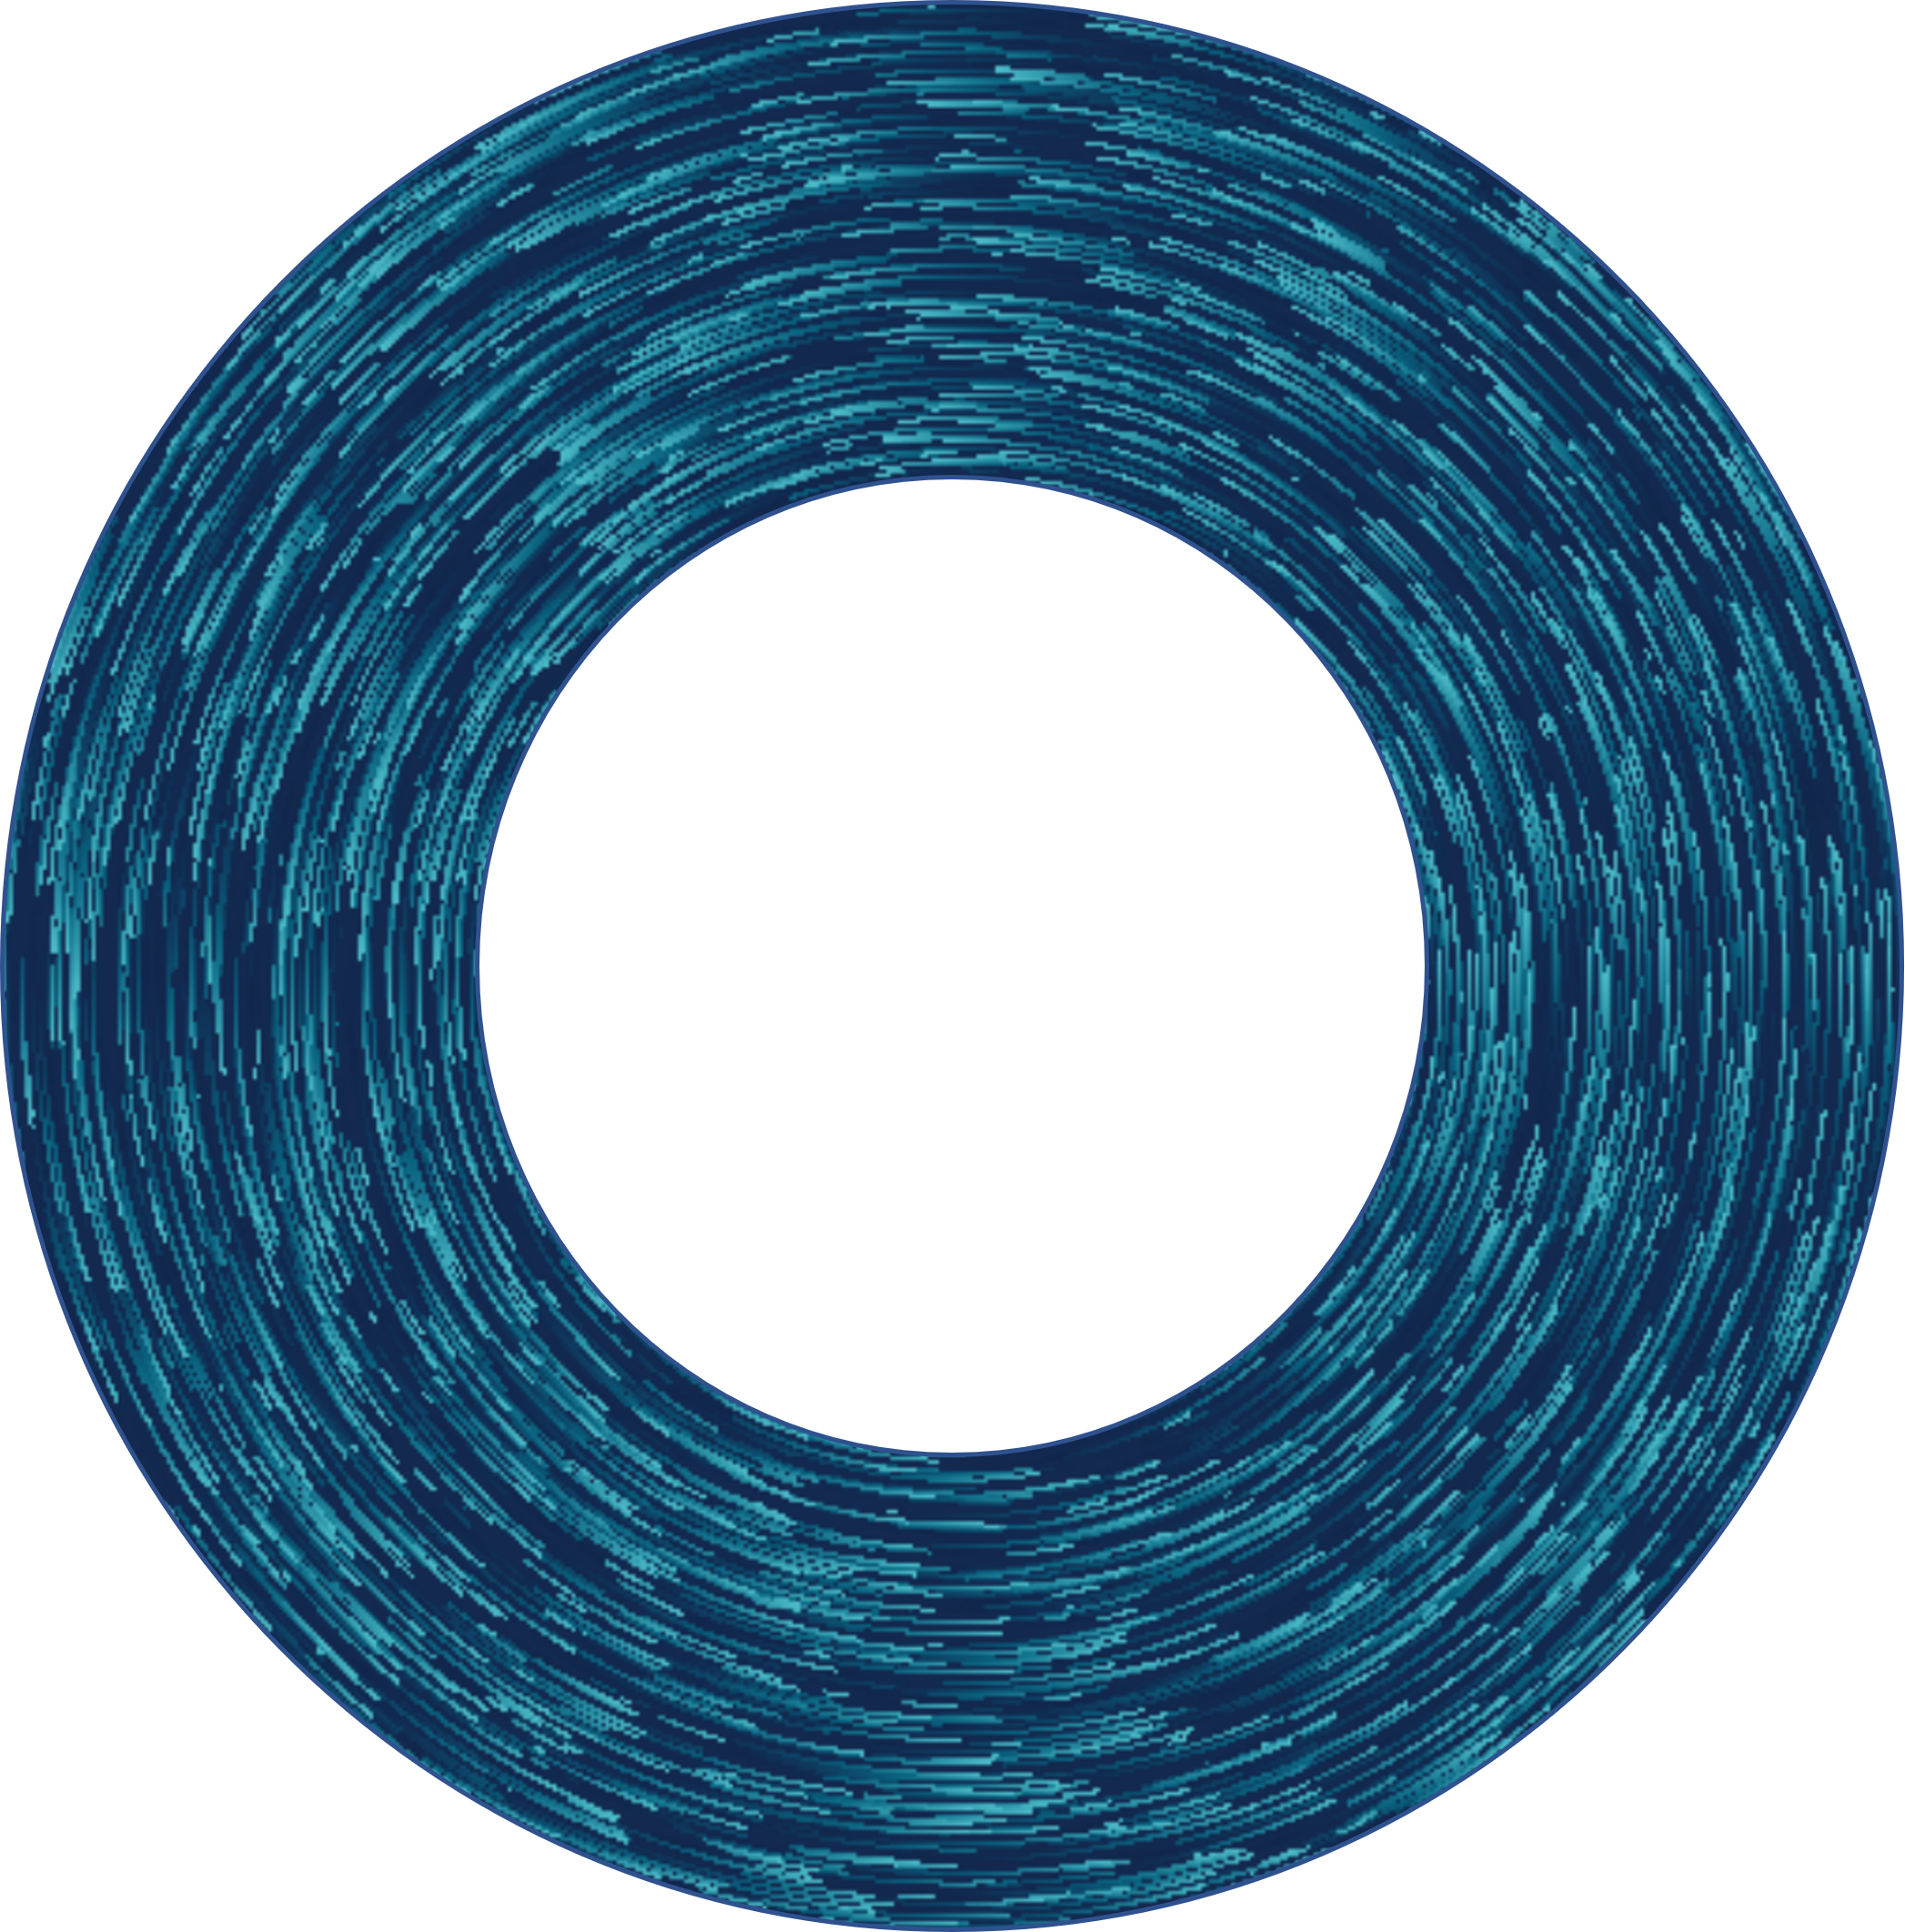
\includegraphics[width=0.4\textwidth]{MeshVectorField.png} 
            \label{fig:example}
            \caption{{\it Left:} Exact solution with mesh. {\it Right:} Magnetic field $\mathbf{b}$.}
        \end{figure}
Mesh has $4709$ nodes.
\end{frame}
    % --- END slide ----
    % --- START slide ----
    \begin{frame}
        \frametitle{Example 1: Error $||u_h-u||_{L^2(\Omega)}$}
\begin{figure}
            \centering
            \includegraphics[width=0.43\textwidth]{Example_1_Error_All.png} 
            \qquad
            \includegraphics[width=0.43\textwidth]{Example_1_Error_Some.png} 
            \label{fig:example}
            \caption{Comparison of error for each method.}
        \end{figure}
    Dots are numerical simulations. We have $\epsilon_0 = 100/\epsilon$, Its = 100.
    \end{frame}
    
    % --- END slide ----
     % --- START slide ----
    \begin{frame}
        \frametitle{Example 2}
        On $\Omega=\{x,y \in \mathbb{R}, 1 < x^2+y^2 < 4\}$ we have 
\begin{align*}
                -\epsilon^{-1}\Delta_{||}u-\Delta_{\bot}u=& \epsilon^{-1}(16x^2+16y^2 - 20),
 \end{align*}
 with $u = 0$ on $\Gamma$. And
 \begin{equation*}
 \mathbf{b} = \left[
 \begin{matrix}
 x \\
 y 
 \end{matrix}
 \right]/\sqrt{x^2+y^2}.
 \end{equation*}
 This has solution
 \begin{equation*}
 u = (x^2+y^2-1)(4-x^2-y^2).
 \end{equation*}
    This is an example problem where all our proposed methods work well.
    \end{frame}
    % --- END slide ----
    % --- START slide ----
    \begin{frame}
        \frametitle{Example 2: Mesh \& Magnetic Field $\mathbf{b}$}
\begin{figure}
            \centering
            \includegraphics[width=0.4\textwidth]{Exact_Solution_Mesh.png} 
            \qquad
            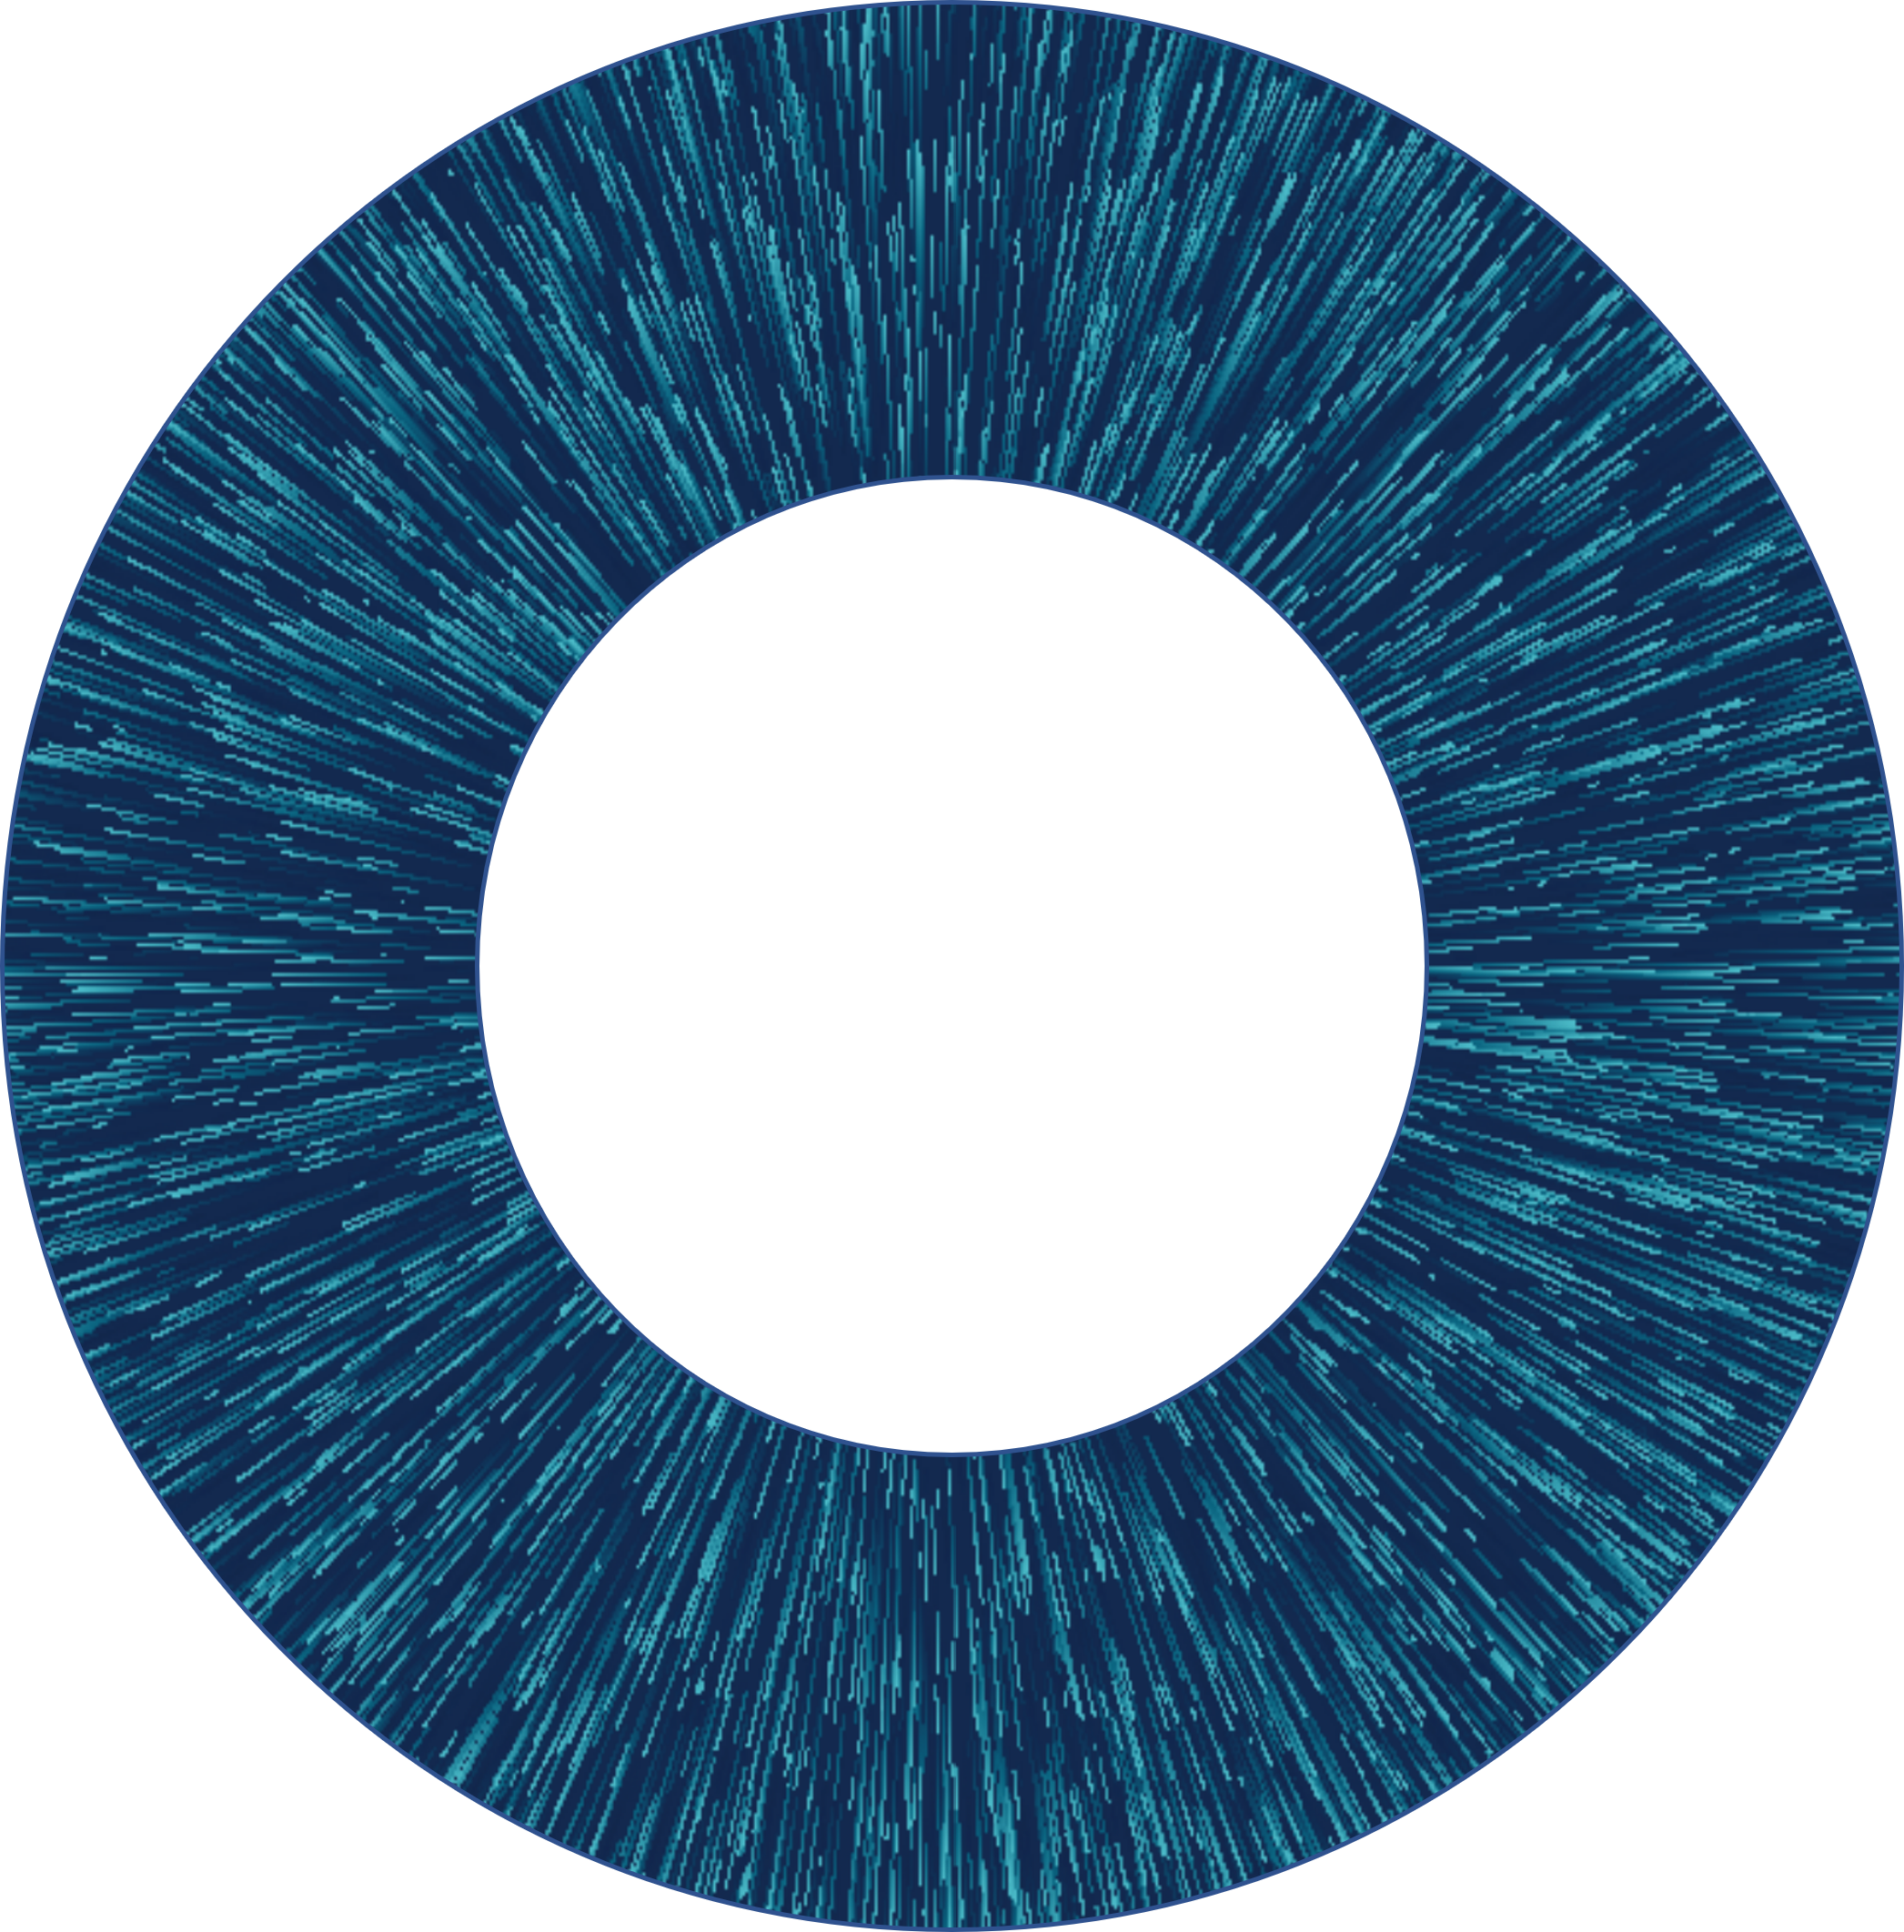
\includegraphics[width=0.4\textwidth]{MeshVectorField2.png} 
            \label{fig:example}
            \caption{{\it Left:} Exact solution with mesh. {\it Right:} Magnetic field $\mathbf{b}$.}
        \end{figure}
Mesh has $4709$ nodes.
\end{frame}
    % --- END slide ----
    % --- START slide ----
    \begin{frame}
        \frametitle{Example 2: Error $||u_h-u||_{L^2(\Omega)}$}
\begin{figure}
            \centering
            \includegraphics[width=0.6\textwidth]{Example_2_Error_Correct.png} 
            \caption{Comparison of error for each method}
        \end{figure}
    Dots indicate numerical simulations. We have $\epsilon_0 = 100\epsilon$, Its = 10.
    \end{frame}
    
    % --- END slide ----
   
    
       % --- START slide ----
    \begin{frame}
        \frametitle{Discussed}
        \begin{itemize}
        \item We have discussed an Iteration method by D\&N, an Alt method and an Expansion around $\epsilon$ method. Then we demonstrated these methods on an Annulus. 
            \item The current methods proposed in this presentation provide a good start. The best being the Alt and D\&N iteration methods. But Culham wants more accuracy.
            \item In the examples convergence stalls. Therefore, to get a better solution increase mesh size.
        \end{itemize}

    \end{frame}
    % --- END slide ----
    
           % --- START slide ----
    \begin{frame}
        \frametitle{The Plan And Questions}
        \begin{itemize}
            \item Find new methods to robustly solve problems like example 1.
            \item Experiment with different finite elements.
            \item See if the expansion around $\epsilon$ method has potential. 
            \item For the Iteration Method, find how to pick $\epsilon_0$.
            \item For the Alt method find a way of implementing the restriction $\mathbf{b}\cdot \nabla_{||}u = 0$ in code. 
            \item Implement methods for spherical tokamak. Therefore, solve on 3D mesh.
\item Prove each method is well posed.
        \end{itemize}

    \end{frame}
    % --- END slide ----
    
\end{document}
